% Op icon: linear pattern (two-tone) - the original (accent) and neutral copies along an arrow.
\documentclass[tikz,border=2mm]{standalone}
\usetikzlibrary{arrows.meta,calc,shapes.geometric}
\begin{document}
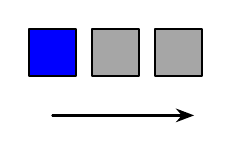
\begin{tikzpicture}[line width=1.3pt, line cap=round, line join=round, >=Stealth, x=1mm,y=1mm]
  \draw[thick, fill=blue] (-12,-3) rectangle (-6,3);
  \draw[thick, fill=gray!70] (-4,-3) rectangle (2,3);
  \draw[thick, fill=gray!70] (4,-3) rectangle (10,3);
  \draw[->, thick] (-9,-8) -- (9,-8);
\end{tikzpicture}
\end{document}
